\section{IEEE 802.15.4e}\label{sec:etat_art-802.15.4}
\renewcommand{\rightmark}{IEEE 802.15.4e}
    802.15.4 est un protocole défini par IEEE en 2003. Il est destiné aux communications à faible débit réalsisées par des dispositifs ayant une alimentation en énergie limitée.
    Ce protocole qui est un standard pour les réseaux PANs (Personal Area Networks) couvre la couche physique et MAC du modèle OSI. En 2012, IEEE 802.15.4e a été défini pour palier certains problèmes de IEEE 802.15.4.

  \subsection*{Types de noeuds et topologie}
    Cette norme définit deux types de noeuds: les Full Function Devices (FFD) qui peuvent être des coordinateurs de PAN, de simple coordinateurs ou de simple noeuds et les Reduced Function Devices (RFD) qui utilisent une implémentation réduite du protocole et ne peuvent être que de simples noeuds.

    Ces noeuds peuvent former des réseaux suivantes plusieurs topologies
    comme la topologie en étoile pour laquelle plusieurs RFD sont connectés à un FFD qui
    joue le rôle de coordinateur ou encore la topologie peer-to-peer pour laquelle les FFD sont connectés les uns aux autres.

  \subsection*{Modes d'accès}
    La norme 802.15.4 définit en 2003 fournit deux modes d'accès: Beacon Enabled mode et Non-Beacon Enabled mode.
    Dans le premier, le réseau est synchronisé par des messages de contrôles (beacons)
    et une structure appelée Superframe.

    Comme l'illustre la figure~\ref{fig:etat_art-802.15.4.superframe}, Cette Superframe est divisée en deux périodes: la période active et la période inactive. La période active est elle-même divisée en deux périodes: contention acces period (CAP) et contention free period (CFP). Dans la première, l'accès au canal se fait par l'algorithme slotted CSMA-CA (Carrier Sense Multiple Access with Collision Avoidance).
    
    Dans la deuxième, l'accès au canal se fait par TDMA (Time Division Multiple Access). C'est à dire que les 7 slots de cette période sont attribués par le coordinateur aux noeuds ayant émis une requête durant la CAP pour l'utilisation d'un slot.

    \begin{figure}[H]
        \centering
        \makebox[\textwidth]
        {
          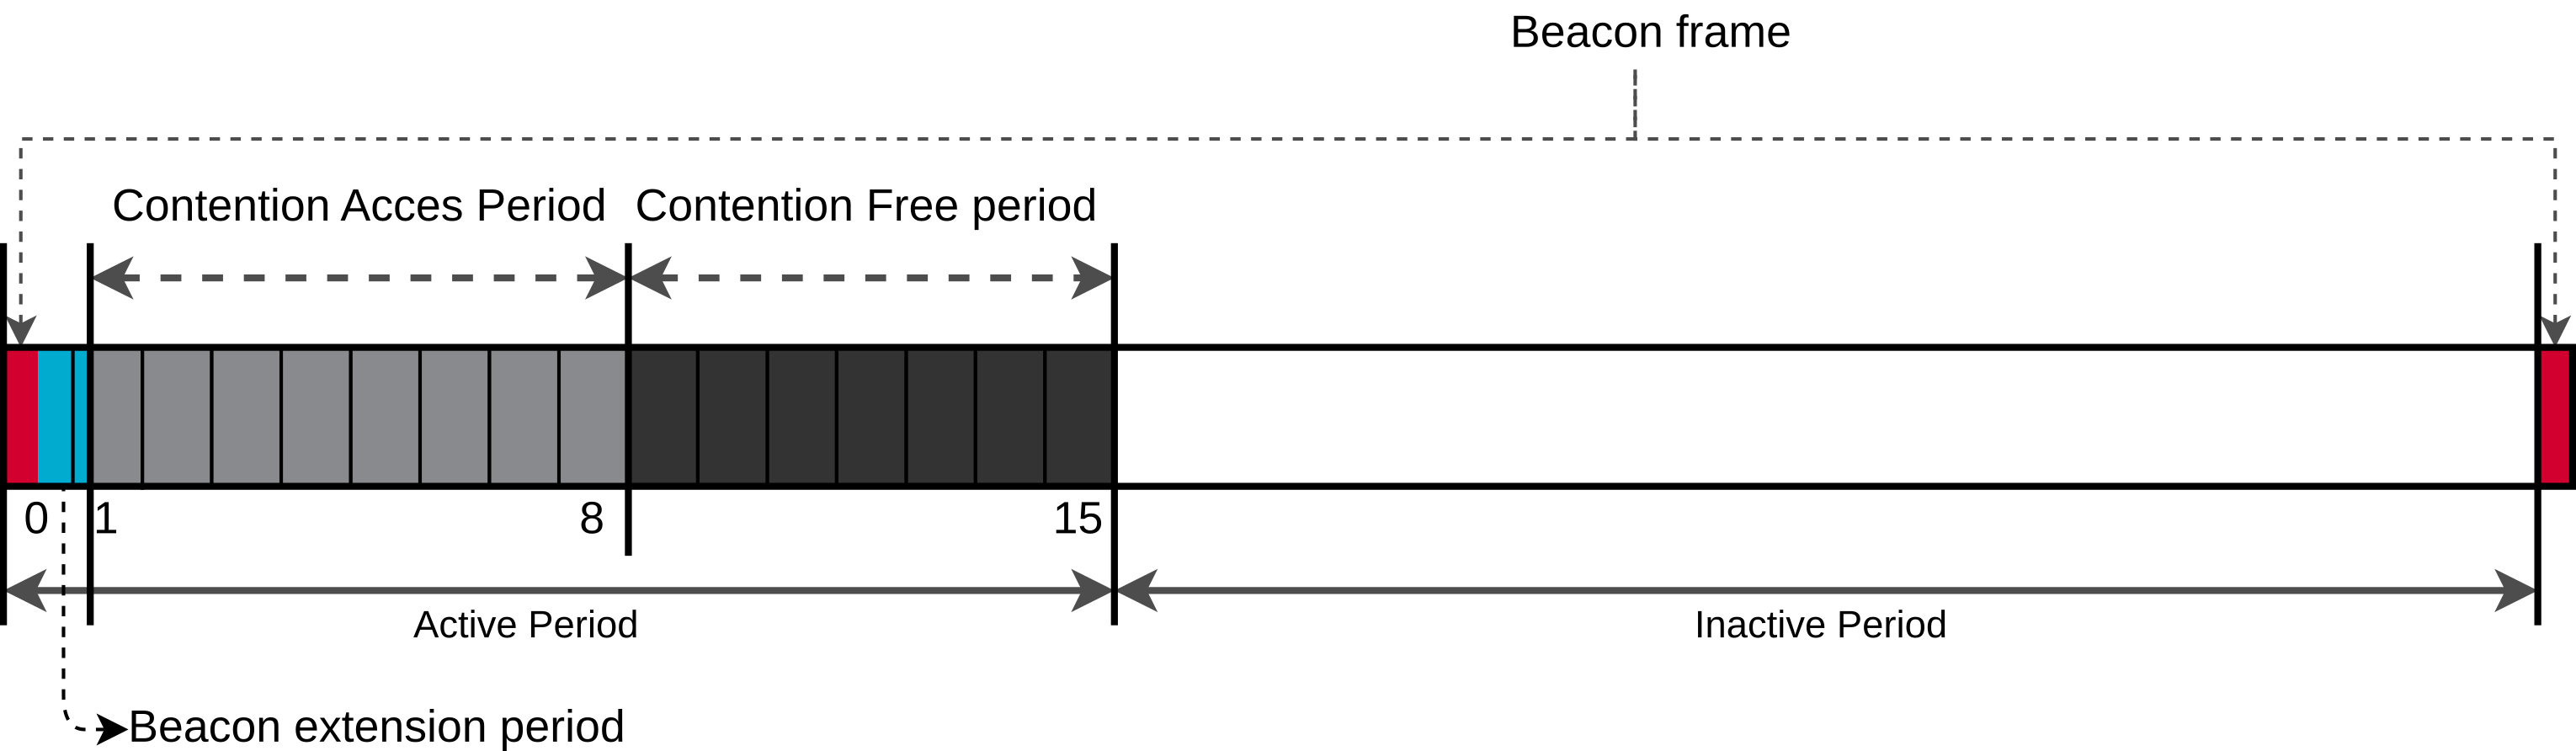
\includegraphics[scale=0.8]{res/pictures/superframe.png}
        }
        \caption{802.15.4 structure de la Superframe.}
        \label{fig:etat_art-802.15.4.superframe}
    \end{figure}

    Dans le mode Non-Beacon Enabled, il n'y a pas de synchronisation. l'accès au canal se fait par l'algorithme Unslotted CSMA-CA.\par


    Ces modes d'accès ont un certains nombres de limitations discutées dans l'article de Domenico De Guglielmo et ses co-auteurs~\cite{paper:802.15.4e-survey}:
    
    \begin{itemize}
      \item Aucune garantie sur le délai maximal pour qu'un paquet puisse atteindre sa destination
        ne peut être fourni avec l'algorithme CSMA-CA.
      \item La fiabilité des communications est limitée par l'utilisation de l'algorithme slotted   CSMA-CA qui offre un taux de transmission faible.
      \item Aucune protection contre les interférences en raison de l'utilisation d'un seul canal et en l'absence de mécanismes de sauts de fréquence (frequency hopping)
    \end{itemize}
    Ces limitations ont menés à la création de 802.15.4.e en 2012 qui redifinit les protocoles MAC du  standard.
    Ainsi, 5 modes de fonctionnement de la couche MAC sont introduits:
    \begin{enumerate}
      \item Time Slotted Channel Hopping (TSCH)
        %Cible les applications tel que l'automatisation de processus. Permet des communications    %multi-sauts et multi-canaux.
      \item Deterministic and Synchronous Multi-channel Extension (DSME)
        %Réalisé pour des applications industirelles et commercialesayant des contraintes de délai et
        %fiabilité. Permet des communications multi-sauts ainsi que la création de réseaux MESH.
      \item Low Latency Deterministic Network (LLDN)
        %Conçu pour les applications nécessitant une latence faible et les réseaux n'utilisant qu'un seul
        %canl pour des chemins d'un saut maximum.
      \item Asynchronous multi-channel adaptation (AMCA)
        %Cible les applications où de grands déploiments sont nécessaire comme le monitoring    %d'infrastructures.
      \item Radio Frequency Identification Blink (BLINK)
        %Conçu pour i'identification de personnes ou d'objets. Il permet aux noeuds de communiquer leur
        %ID aux autres noeuds sans avoir été préalablement associés.
    \end{enumerate}
    D'après l'article de Domenico De Guglielmo et ses co-auteurs~\cite{paper:802.15.4e-survey}, le standard ne définit que brièvement AMCA et BLINK.
    LLDN est destiné aux réseaux à un seul saut et utilisant un seul canal. Il n'est donc pas pertinent pour ce projet. DSME utilise le concept de multi-superframe semblable aux superframes de IEEE 802.15.4 mis à part la CFP qui divise chacun des 7 slots en plusieurs fréquences.


\subsection*{TSCH (Time Slotted Channel Hopping)}\label{subsec:etat_art-802.15.4.tsch}

Ce mode de fonctionnement de la couche MAC, comme son nom l'indique, supporte à la fois les sauts en fréquence et des communications divisées en temps. Ces mécanismes réduisent efficacement les effets des interférences et les collisions ce qui améliore la fiabilité du réseau.

\subsubsection*{Slotframe}
Dans ce mode, le concept de superframe de 802.15.4 est remplacé par le concept de slotframe.
Une slotframe est un intervalle de temps qui est divisé en timeslots et se répète infiniment. Chaque timeslot permet à un noeud d'envoyer une trame et d'éventuellement recevoir son acquitement (ACK).
Chaque timeslot possède un identifiant appellé \textit{Absolute Slot Number} (ASN)
et un identifiant au sein de la slotframe appelé \textit{Time Slot Number} (TSN).

TSCH permet l'utilisation de timeslots partagés et dédiés. Dans les timeslots partagés plusieurs noeuds peuvent communiquer. Dans ce cas, CSMA/ CA est utilisé. Pour les timeslots dédiés, seuls deux noeuds peuvent communiquer. La figure~\ref{fig:state-slotframe} illustre une slotframe composée de trois timeslots.
Dans cet exemple, on considère 3 noeuds: N, T et U. Chaque timeslot permet une communication entre deux noeuds.
Par exemple le timeslot ayant comme TSN 0, permet à N de transmettre vers T.

\begin{figure}[H]
  \centering
  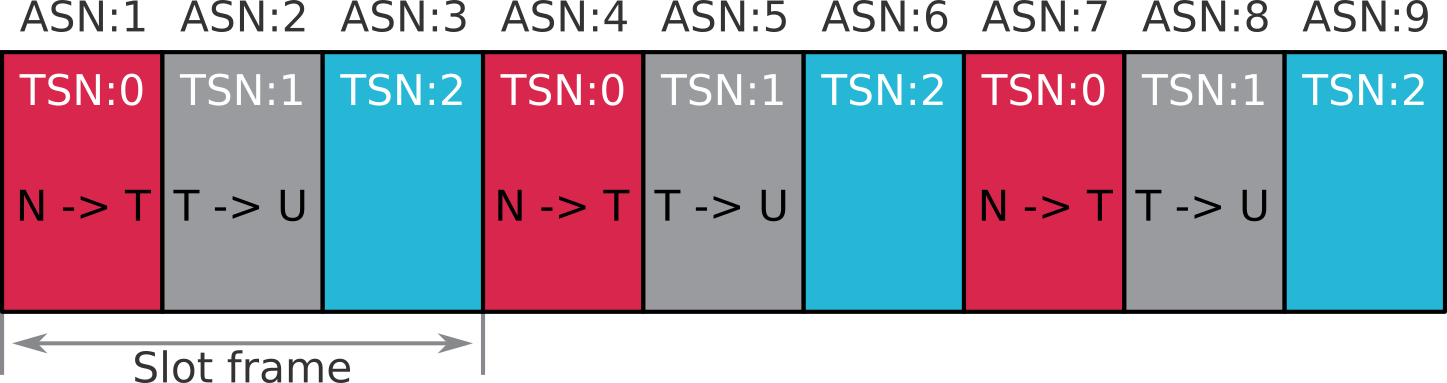
\includegraphics[scale=0.7]{res/pictures/sloframe.png}
  \caption{Exemple de Slotframe.}
  \label{fig:state-slotframe}
\end{figure}

\subsubsection*{Channel Hopping}

TSCH peut utiliser 16 canaux différents. Un lien entre deux noeuds dans TSCH est alors défini par la paire (timeslot, canal). Ainsi, chaque slotframe est divisée par le nombre de canaux utilisés dans le réseau (Fig.~\ref{fig:state-tsch}). La fréquence $f$ utilisée pour la communication entre deux noeuds est calculée comme suit:

\[
    f = F[(ASN + channel Offset)\% N_{channels}]
\]

où $N_{channels}$ est le nombre de canaux utilisés pour le réseau et F peut être vue comme une table qui contient une permutation pseudo-aléatoire de canaux.

\begin{figure}[H]
    \centering
    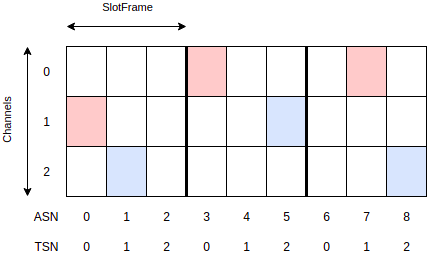
\includegraphics[scale=0.5]{res/pictures/tsch.drawio.png}
    \caption{Time Slotted Channel Hopping.}
    \label{fig:state-tsch}
\end{figure}


%\subsubsection*{Formation du PAN}

%\subsubsection*{Synchronisation en temps}